\chapter{Query Language}
\label{sec:specification_language}

The centre-piece of the \vnnlib{} standard is the \vnnlib{} query language which is heavily inspired by the SMT-LIB query language and is designed as a standardised computer-readable format for expressing satisfiability problems over neural networks.
Although the syntax is somewhat human-readable, the query language is designed to primarily optimise machine-readability. 
It is expected that \vnnlib{} queries will primarily be generated automatically by higher level tools that provide more human-friendly interfaces.
This chapter describes the syntax, scoping, typing and semantics of the query language. Unless explicitly stated otherwise, everything in this chapter is implicitly parameterised by some underlying network theory $\networkTheoryVar$, the definition of which was provided in Section~\ref{sec:network-theory}.

\section{Syntax}
\label{sec:syntax}

\begin{figure}
	\setlength{\grammarindent}{6.5em}
	
	\begin{grammar}
	<query> ::= <version> [<network>]$^+$ [<assert>]$^*$
	
	<version> ::= (\texttt{vnnlib-version} [0-9]$^+$.[0-9]$^+$)
	
	<name> ::= [A-Za-z][\_A-Za-z0-9]*
		
	<network> ::= (\texttt{declare-network} <name> <equiv>$^?$ <input>$^+$ <hidden>* <output>$^+$)
	
	<equiv> ::= (\texttt{equal-to} <name>) | (\texttt{isomorphic-to} <name>)
	
	<input> ::= (\texttt{declare-input} <name> <elementType>$_\networkTheoryVar$ <shape>)
	
	<hidden> ::= (\texttt{declare-hidden} <name> <elementType>$_\networkTheoryVar$ <shape> <name>)
	
	<output> ::= (\texttt{declare-output} <name> <elementType>$_\networkTheoryVar$ <shape>)
	
	<assert> ::= (\texttt{assert} <bool>)
	
	<bool> ::= (\texttt{and} <bool> <bool>$^+$)
	\alt (\texttt{or} <bool> <bool>$^+$)
	\alt (\texttt{+} <arith> <arith>)
	\alt (\texttt{\textless} <arith> <arith>)
	\alt (\texttt{\textless=} <arith> <arith>)
	\alt (\texttt{\textgreater} <arith> <arith>)
	\alt (\texttt{\textgreater=} <arith> <arith>)
	\alt (\texttt{==} <arith> <arith>)
	\alt (\texttt{!=} <arith> <arith>)
	
	<arith> ::= <element>$_\networkTheoryVar$
	\alt <name> <indices>
	\alt (\texttt{-} <arith>)
	\alt (\texttt{+} <arith> <arith>$^+$)
	\alt (\texttt{*} <arith> <arith>$^+$)
	\alt (\texttt{-} <arith> <arith>$^+$)
	
	<indices> ::= [i, ..., i] for $i \in \mathbb{N}$
	\end{grammar}
	\vspace{-1em}
    \caption{The syntax of \vnnlib{} queries, parameterised by the syntax of the underlying network theory $\networkTheoryVar$ described in Figures~\ref{fig:onnx-type-syntax}~\&~\ref{fig:onnx-expr-syntax}. As is convention, $^*$ means zero or more, $^+$ means one or more, and $^?$ means optional.}
    \label{fig:vnnlib-syntax}
\end{figure}

The syntax of the \vnnlib{} query language is shown in Figure~\ref{fig:vnnlib-syntax}.  This section will now describe the key syntactic constructs of the language via illustrative examples. Firstly, queries are split into three parts: 
\begin{enumerate}
\item \textbf{Version number} - the version of the VNN-LIB the query is using. This allows tools to provide better diagnostic error messages.
\item \textbf{Network declarations} - a non-empty list of network declarations. These describe the networks that involved in the satisfiability problem and allow the introduction of new abstract variables that represent the values for the inputs and outputs of those networks.
\item \textbf{Assertions} - a list of assertions that reference the variables introduced by the network declarations, thereby defining the constraints that should be satisfied.
\end{enumerate}
Currently, the standard does not permit the interleaving of network declarations and assertions. Figure~\ref{fig:simple-query} shows an example of a simple query.


\subsection{Network Declarations}
\label{sec:network-declarations}

A network is introduced by the keyword \texttt{declare-network}, followed by a user-defined name for the network, and then declarations for its associated input and output. 
An input is declared using the \texttt{declare-input} keyword, followed by a variable name, an element type from the associated \networkTheory{} (e.g., \texttt{float64}, \texttt{int32}), 
and the shape of the tensor. Similarly, an output variable uses the \texttt{declare-output} keyword. In the case of Figure~\ref{fig:simple-query}, the network is named \texttt{myNetwork}, and it has one input called \texttt{X} consisting of a $1 \times 10$ tensor of ONNX \texttt{float32} values and one output called \texttt{Y} consisting of a $1 \times 2$ tensor of ONNX \texttt{float32} values. 
\begin{figure}[t]
    \begin{minipage}[c]{0.62\textwidth}
        \begin{lstlisting}[style=lbnf]
(declare-network myNetwork
    (declare-input  X float32 [1,10])
    (declare-output Y float32 [1,2])
)

(assert (>= X[0,2] 0.0))
(assert (<= X[0,2] 1.0))
(assert (<= Y[0,1] 0.5))\end{lstlisting}
    \end{minipage}%
    \begin{minipage}[c]{0.35\textwidth}
        \centering
        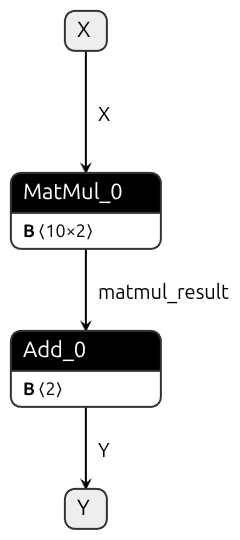
\includegraphics[height=5cm]{imgs/simple_net.onnx.png}
    \end{minipage}
    \caption{A simple \vnnlib{} specification which declares a network with a single input and output tensor. An example of one of the many possible ONNX models compatible with this declaration is shown on the right. Note that the variable names \texttt{X} and \texttt{Y} for the declared inputs and outputs do not have to match the node names in the ONNX model.}
    \label{fig:simple-query}
\end{figure}


All variable names follow the same syntax conventions: they are case-sensitive, must start with a letter, and may only contain letters, digits and underscores. All variable names must be unique within the query (see Section~\ref{sec:scoping_and_typing} for more detailed scoping rules). 


It is important to clarify that a network declaration only declares an \emph{interface} and does not reference any particular ONNX network model. 
When passing a query and a network model to the verifier, the name of the network does not need to match the name of the ONNX model file. 
Instead, as described in Section~\ref{sec:verify_command}, the user will explicitly associate a network declaration to the relevant model file via the command line.
Neither do the declared names of the inputs and outputs need to match the names of the input and output nodes within the ONNX model file. This flexibility allows many different alternative ONNX models to be compatible with the same query.

Equally, the network declarations do not constrain the internal architecture of the model, including which operators (e.g. Gemm, ReLU, Softmax) are used. In practice, different verifiers will support different operators and Section~\ref{sec:onnx-capabilities} provides a mechanism for a verifier to report its own capabilities in this regard.

% The \texttt{@} character is a reserved character which is used to denote multiple applications of the same network, for the purpose of defining  hyperproperties such as monotonicity. For example \texttt{(declare-network acasXu@1 ...)} and \texttt{(declare-network acasXu@2 ...)} define two networks that are both instances of the same ONNX model,  denoted as \texttt{acasXu} in the command line interface of the verifier (See Chapter~\ref{sec:solver_interface} for more details).

\subsection{Assertions}

The list of assertions constrain the variables introduced by the network declarations. \vnnlib{} assertions are quantifier-free logical formulas and are defined using parenthesized \texttt{(assert\ldots)} expressions. 
They use an SMT-LIB-like reverse Polish notation syntax with the operator preceding its operands.
An assertion is a logical formula that may include logical connectives, relational comparisons, and arithmetic expressions over declared tensors and constants.
The final satisfiability problem is then the conjunction of all the assertions.
 
\paragraph{Constants}

Numeric constant values may be referenced using basic standard integer or floating point syntax (e.g. \inlinevnn{0}, \inlinevnn{0.0}, \inlinevnn{-0.5}). 

\paragraph{Variables} 

Standard indexing notation may be used to refer to a specific element within the tensor variable. For example, Line 6 in Figure~\ref{fig:simple-query} uses \inlinevnn{X[0,2]}, to refer to the value of the element of the input tensor at row~0, column~2. All indices are zero based and currently the number of indices provided must be equal to the number of dimensions of the variable, i.e. partial indexing is not allowed.

\paragraph{Arithmetic expressions}

One forms arithmetic expressions by recursively combining constant and variable values via prefix notation. Currently the following operators are supported:
\begin{itemize}
	\item \inlinevnn{(- a)}: Negation of a term.
    \item \inlinevnn{(+ a b ...)}: Addition of two or more terms. 
    \item \inlinevnn{(* a b ...)}: Multiplication of two or more terms. 
    \item \inlinevnn{(- a b ...)}: Subtraction of two or more terms. Note that subtraction associates to the left, e.g. \inlinevnn{(- 1 2 3 4)} is the same as \inlinevnn{(- (- (- 1 2) 3) 4)} .
\end{itemize}
Arithmetic operations currently only operate over individual tensor elements and cannot be used to operate over multi-dimensional tensors (see Section~\ref{sec:scoping_and_typing} for detailed typing rules). 

Although some ONNX types can be safely coerced between in certain cases (e.g. a \inlinevnn{float16} can be added safely to a \inlinevnn{float32} if the expected type of evaluated expression is a \inlinevnn{float32}), the \vnnlib{} standard does not permit such coercions.
All variables within an arithmetic expression must have the same type (see Section~\ref{sec:scoping_and_typing} for formal typing rules). 

\paragraph{Comparisons}

The comparison operators \inlinevnn{<=}, \inlinevnn{>=}, \inlinevnn{<}, \inlinevnn{>}, \inlinevnn{=}, \inlinevnn{!=} can be used to compare the values of two arithmetic operations.
For example, \inlinevnn{(<= a b)} returns true if $a$ is less than or equal to $b$.
    
\paragraph{Boolean expressions} 

One forms boolean expressions by recursively combining comparisons via the following supported logical connectives:
\begin{itemize}
    \item \inlinevnn{(and a b ...)}: Conjunction of two or more terms.
    \item \inlinevnn{(or a b ...)}: Disjunction of two or more terms.
\end{itemize}

\subsection{Complex Network Declarations}
\label{sec:complex-networks-decls}

Although queries often relate the input of a single network to its output in some way, \vnnlib{} supports more complex queries. The neural network may have multiple input or output nodes, or the query may refer to intermediate hidden layers of the network or it may relate the behaviour of multiple networks. The query language supports all of these use cases.

\subsubsection{Multiple input and output declarations}

Neural network that accept multi-modal input or produce multi-modal output are becoming increasingly common. 
For example, the network in Figure~\ref{fig:multi-inputs-outputs} shows a model that takes both an image and meta-data about that image as inputs, and outputs both a bounding box around an identified object of interest and a probability distribution over the possible class that the object belongs to. 

The query language supports such networks by allowing a network declaration to declare an arbitrary number of input and output declarations. The question is then how is the list of declared inputs and outputs mapped to the list of inputs and outputs nodes in the ONNX model. There are two ways to specify this mapping: 
\begin{itemize}
    \item \textbf{By order:} the default is that declared inputs and outputs are mapped to the ONNX graph's inputs and outputs by matching the order of declaration in the query to the order of declaration in the ONNX model file. This is demonstrated in the top code snippet in Figure~\ref{fig:multi-inputs-outputs}
    \item \textbf{By name:} alternatively, variables can be explicitly mapped using the names of the nodes within the ONNX graph. If this method is used, all input and output variables within that network declaration must be given an explicit ONNX node name. This is demonstrated in the bottom code snippet in Figure~\ref{fig:multi-inputs-outputs}.
\end{itemize}

\begin{figure}[h!]
    \centering
    \begin{lstlisting}[style=lbnf]
(declare-network multi_io_net
    (declare-input  image    float32 [1,3,224,224])
    (declare-input  metadata float32 [1,10])
    (declare-output bbox     int16   [1 4])
    (declare-output logits   float32 [1,1000])
)\end{lstlisting}

    \begin{lstlisting}[style=lbnf]
(declare-network multi_io_net
    (declare-input  metadata float32 [1,10]        "metadata")
    (declare-input  image    float32 [1,3,224,224] "image")
    (declare-output logits   float32 [1,1000]      "logits")
    (declare-output bbox     int16   [1,4,2]       "bbox")
)\end{lstlisting}

    \vspace{0.5cm}
    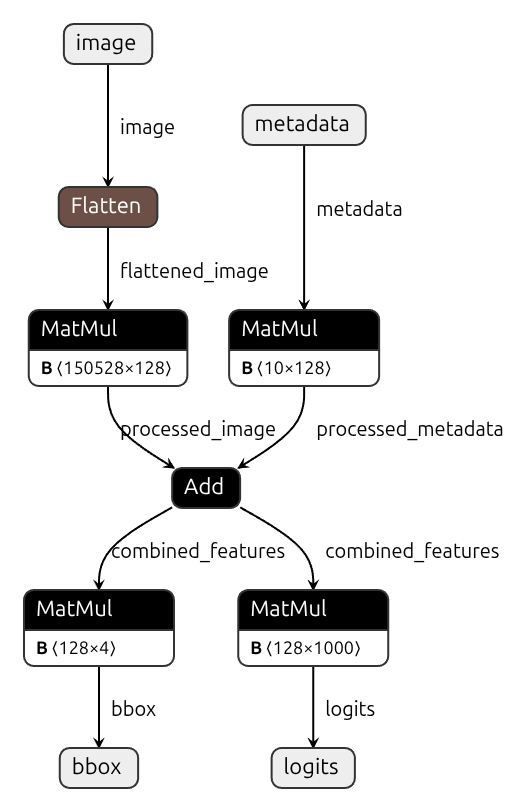
\includegraphics[width=\textwidth]{imgs/multi_io_net.onnx.png}
    \caption{A \vnnlib{} network declaration with multiple inputs/outputs. The first code snippet shows the declared inputs and outputs mapped to the ONNX inputs and outputs nodes by declaration order, while the second snippet shows them explicitly mapped by the name of the ONNX node.}
    \label{fig:multi-inputs-outputs}
\end{figure}


\subsubsection{Hidden output declarations}
\label{sec:hidden-output-declarations}

In some use cases it is desirable to constrain the result of intermediate computation at the output of hidden nodes within the network. For example, when reasoning about the encodings in an encoder-decoder architecture or when reasoning about attention mechanisms. This can be achieved by declaring hidden nodes using the \texttt{declare-hidden} keyword. This declaration includes a variable name for use within the \vnnlib{} specification,  its element type, its tensor shape, and crucially, a string identifier that specifies the corresponding node name in the ONNX graph.  Multiple hidden nodes can be trivially declared within a single network declaration. Figure~\ref{fig:hidden-node} shows a \vnnlib{} network declaration with a hidden node.

\begin{figure}[h!]
    \begin{minipage}[c]{0.76\textwidth}
        \begin{lstlisting}[style=lbnf]   
(declare-network encoder
    (declare-input  X float64 [1,28,28])
    (declare-hidden Z float64 [1,128] "hidden")
    (declare-output Y float64 [1,10])
)\end{lstlisting}
    \end{minipage}%
    \begin{minipage}[c]{0.21\textwidth}
        \centering
        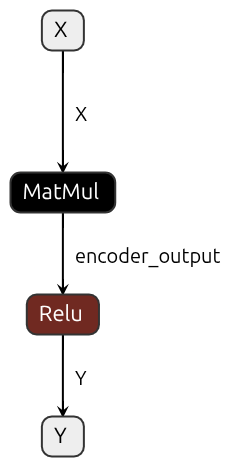
\includegraphics[height=6cm]{imgs/encoder_net.onnx.png}
    \end{minipage}
    \caption{A \vnnlib{} network declaration that declares a hidden node}
    \label{fig:hidden-node}
\end{figure}

The hidden node declaration crucially refers to the uniquely identified outputs of a node, rather than the node (or operator) itself. It declares that an output of the node is to be used as a variable in the \vnnlib{} query.

\subsubsection{Multiple networks}
\label{sec:multiple-network}

Often you may want to relate the behaviour of one neural network to that of another. Classic examples include: teacher-student networks where you try to train a smaller, more efficient network to mimic the output of the larger network, or observer-controller architectures.

\vnnlib{} supports defining multiple networks in by including multiple network declarations in the same query. Figure~\ref{fig:multiple-networks} 
shows an example which declares two networks representing a teacher and a student network.

\begin{figure}[h!]
    \begin{minipage}[c]{0.64\textwidth}
        \begin{lstlisting}[style=lbnf]
(declare-network teacher
    (declare-input  TX float32 [1,32])
    (declare-output TY float32 [1,2])
)

(declare-network student
    (declare-input  SX float16 [1,32])
    (declare-output SY float16 [1,2])
)\end{lstlisting}
    \end{minipage}
    \begin{minipage}[c]{0.35\textwidth}
        \centering
        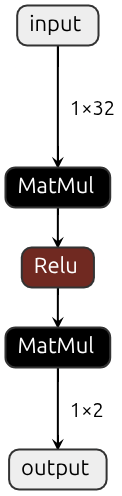
\includegraphics[height=7cm]{imgs/teacher_net.onnx.png}
        \vspace{0.5cm} 
        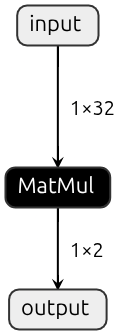
\includegraphics[height=5cm]{imgs/student_net.onnx.png}
    \end{minipage}
    \caption{A pair of \vnnlib{} network declarations that allows the referencing of multiple networks within a single query.}
    \label{fig:multiple-networks}
\end{figure}

For some use cases involving multiple networks (e.g. proving monotonicity), each \texttt{declare-network} declaration is intended to map to the same network implementation. In this case, the \texttt{equal-to} declaration may be used as shown in Figure~\ref{fig:multiple-equal-networks} to inform the verifier of this fact. An \texttt{equal-to} declaration must reference a network declaration which has identical \texttt{declare-input} and \texttt{declare-output} declarations (modulo the variable names). It \emph{is} possible to have a different list of \texttt{declare-hidden} declarations in the two networks. However if a \texttt{declare-hidden} declaration that references the same ONNX node is present in both networks then those \texttt{declare-hidden} declarations must be identical modulo the variable names. 
 Finally, marking a \texttt{declare-network} declaration as equal to one another means that it is not necessary to provide an implementation for that declaration when calling the verifier (see Section~\ref{sec:verify_command} for details).
 
\begin{figure}[h!]
    \begin{minipage}[c]{0.64\textwidth}
        \begin{lstlisting}[style=lbnf]
(declare-network f
    (declare-input  A float32 [1,10])
    (declare-output B float32 [1,2])
)

(declare-network f-copy
    (equal-to f)
    (declare-input  C float32 [1,10])
    (declare-output D float32 [1,2])
)\end{lstlisting}
    \end{minipage}
    \begin{minipage}[c]{0.35\textwidth}
        \centering
        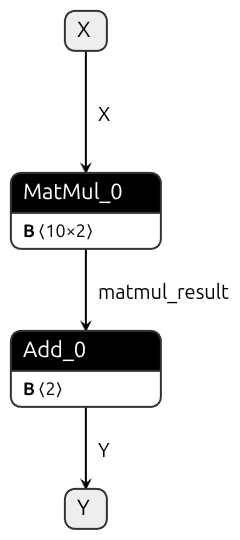
\includegraphics[height=5cm]{imgs/simple_net.onnx.png}
    \end{minipage}
    \caption{A pair of \vnnlib{} network declarations that reference the same ONNX network.}
    \label{fig:multiple-equal-networks}
\end{figure}

In other use cases involving multiple networks (e.g. proving local equivalence after retraining or after quantisation), each network declaration will be mapped to a network with the same graph structure but with different weights. In this case, the \texttt{isomorphic-to} declaration may be used as shown in Figure~\ref{fig:multiple-isomorphic-networks}. An \texttt{isomorphic-to} declaration must reference a network declaration which has identical list of \texttt{declare-input} and \texttt{declare-output} declarations, modulo the variable names and the element type. As with the \texttt{equal-to} declaration, it \emph{is} possible to have a different list of \texttt{declare-hidden} declarations in the two \texttt{declare-network} declarations. However if a \texttt{declare-hidden} declaration that references the same ONNX node is present in both then those \texttt{declare-hidden} declarations must be identical modulo the variable names and element types.

\begin{figure}[h!]
    \begin{minipage}[c]{0.64\textwidth}
        \begin{lstlisting}[style=lbnf]
(declare-network f
    (declare-input  A float32 [1,10])
    (declare-output B float32 [1,2])
)

(declare-network g
    (isomorphic-to f)
    (declare-input  C float32 [1,10])
    (declare-output D float32 [1,2])
)\end{lstlisting}
    \end{minipage}
    \begin{minipage}[c]{0.35\textwidth}
        \centering
        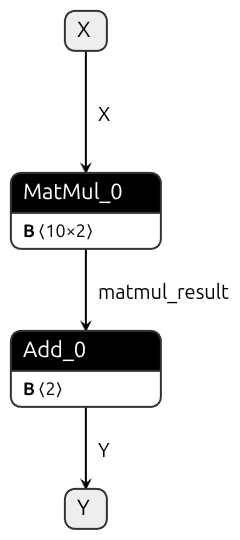
\includegraphics[height=5cm]{imgs/simple_net.onnx.png}
        \vspace{0.5cm} 
        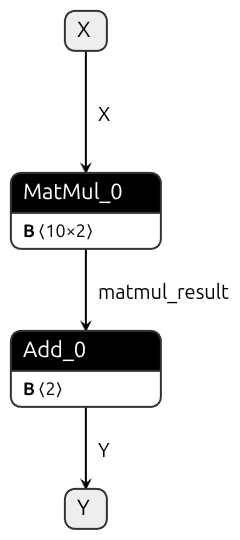
\includegraphics[height=5cm]{imgs/simple_net.onnx.png}
    \end{minipage}
    \caption{A pair of \vnnlib{} network declarations that reference isomorphic ONNX networks.}
    \label{fig:multiple-isomorphic-networks}
\end{figure}

There are two additional restrictions to their use:
\begin{enumerate}
\item A \texttt{declare-network} declaration must contain at most one \texttt{equal-to} or \texttt{isomorphic-to} declaration.
\item An \texttt{equal-to} or \texttt{isomorphic-to} declaration cannot reference another network declaration that also contains an \texttt{equal-to} or \texttt{isomorphic-to}. 
\end{enumerate}
Due to the transitivity of equality and isomorphism, these restrictions do not reduce the expressive power of this feature, and make the dependencies easier to track by the verifiers.

While a verifier may make use of the \texttt{equal-to} and \texttt{isomorphic-to} declarations internally to optimise its representation and reasoning about the provided networks, it is not required to.



\subsection{Comments and Whitespace}

Comments in \vnnlib{} are denoted by a semicolon (\texttt{;}) and extend to the end of the line. They are used for annotation, explaining logic, or providing additional context. Whitespace in \vnnlib{} is used to separate tokens and improve readability and can include spaces, tabs, and newlines. Additional whitespace beyond the minimal necessary to separate tokens is ignored.


\section{Typing}
\label{sec:scoping_and_typing}

This section describes the typing rules for \vnnlib{} queries. The rules provide a formal description of the constraints on the syntax described informally in Section~\ref{sec:syntax}, e.g. all variable names must be unique, variables of different types cannot appear in the same assertion. 

Crucial to the typing rules is the notion of the current \emph{context} $\assertCtx = (\networkCtx, \variableCtx)$ which consists of two parts. The first is the \emph{network context}, $\networkCtx : \mgrammar{<name>} \rightarrow \mgrammar{<network>}$, which is a mapping from network names to the corresponding network declarations. The second is the \emph{variable context}, $\variableCtx : \mgrammar{<name>} \rightarrow \mgrammar{<tensorType>}_\networkTheoryVar$, which is a mapping from the decared input/hidden/output variables to their shape and type.

As one would expect, queries are typed  by first constructing the context $\assertCtx$ by iterating over the network declarations, and then using that context to type the globally-scoped assertions:
\begin{mathpar}
            \inferrule*[Right=Query]
            {
            	{\begin{array}{ll}
	            \emptyset &
	            \vdash \networkDeclVar_1 : \assertCtx_1 \\
	            \assertCtx_{1} &
	            \vdash \networkDeclVar_2 : \assertCtx_2 \\
                & \vdots \\
	            \assertCtx_{n-1} &
	            \vdash \networkDeclVar_n : \assertCtx_n
	            \end{array}}
	            \\
	            {\begin{array}{ll}
                \assertCtx_n &
                \vdash \assertionVar_1 \\
                \assertCtx_n &
                \vdash \assertionVar_2 \\
                &\vdots \\
                \assertCtx_n &
                \vdash \assertionVar_m
                \end{array}}
            }
            {
                \vdash \queryExpansion
            }
\end{mathpar}

The following sections now describe the typing rules for network declarations and assertions.

\subsection{Networks}

The rule for typing a network declaration is as follows:
\begin{mathpar}
    \inferrule*[]
    {
        {\begin{array}{c}
        \nameVar \notin \networkCtx
        \hspace{1em}
        {\color{red} e???} 
        \vspace{1.5em}
        \\
        \vspace{0.25em}
        {
            \begin{array}{lll}
                \variableCtx_0 &
                \vdash \inputDeclVar_1 : \variableCtx_1 
                \\
                &\vdots
                \\
                \variableCtx_{n-1} &
                \vdash \inputDeclVar_n : \variableCtx_n 
            \end{array}
        }
        \hspace{1em}
        {
            \begin{array}{lll}
                \variableCtx_n &
                \vdash \hiddenDeclVar_1 : \variableCtx_{n+1} 
                \\                    
                &\vdots 
                \\                    
                \variableCtx_{m+n-1} &
                \vdash \hiddenDeclVar_m : \variableCtx_{m+n} 
            \end{array}
        }       
        \hspace{1em}         
        {
            \begin{array}{lll}
                \variableCtx_{m+n} &
                \vdash \outputDeclVar_1 : \variableCtx_{m+n+1} 
                \\
                &\vdots
                \\
                \variableCtx_{m+n+o-1} &
                \vdash \outputDeclVar_o : \variableCtx_{n+m+o} 
            \end{array}
        }
        \end{array}}
    }
    {
        \networkCtx, \variableCtx 
        \vdash \networkExpansion : 
        \networkCtx[\nameVar \rightarrow ..], \variableCtx_{n+m+o+1}
    }
\end{mathpar}

First it is checked that the network name is unique, next the variable context is updated by iterating sequentially through the input, hidden and output node declarations. 

The rules for typing input/hidden and output declarations are as follows:
\begin{mathpar}
            \inferrule*[Right=Input]
            {
            	v \notin \variableCtx
            }
            {
                \variableCtx \vdash \texttt{declare-input}~v~\tau~s : \variableCtx[v \rightarrow (\tau, s)]
            }
            \\
            \inferrule*[Right=Hidden]
            {
            	v \notin \variableCtx
            }
            {
                \variableCtx \vdash \texttt{declare-hidden}~v~\tau~s~n : \variableCtx[ v \rightarrow (\tau, s)]
            }
            \\
            \inferrule*[Right=Output]
            {
            	v \notin \variableCtx
            }
            {
                \variableCtx \vdash \texttt{declare-output}~v~\tau~s : \variableCtx[ v \rightarrow (\tau, s)]
            }
\end{mathpar}

i.e. as long as the name of the variable has not already been seen and is therefore unique, then each declaration  adds a corresponding entry to the $\variableCtx$.

\subsection{Assertions}

Assertions are type-checked within some variable context.
\begin{mathpar}
    \inferrule*[Right=Assertion]
    {
        \assertCtx \vdash b
    }
    {
        \assertCtx \vdash (\texttt{assert}~b)
    }
\end{mathpar}

which simply defers to the typing of boolean expressions.

The boolean expressions consist of the n-ary operations \texttt{and} and \texttt{or}, and the six comparison operators which can be type-checked as follows:
\begin{mathpar}
    \inferrule*[Right=Comparison]{
        \assertCtx \vdash a_1 : \tau \quad \assertCtx \vdash a_2 : \tau \quad \lozenge \in \{\texttt{>=}, \texttt{>}, \texttt{<}, \texttt{<=}, \texttt{==}, \texttt{!=}\}
    }{
        \assertCtx \vdash \lozenge~a_1~a_2
    }
    \\
    \hspace{1cm}
    \inferrule*[Right=N-ary Boolean]{
        \assertCtx \vdash b_1 \quad ... \quad \assertCtx \vdash b_n \quad \lozenge \in \{\texttt{and}, \texttt{or}\}
    }{
        \assertCtx \vdash \lozenge~b_1~...~b_n
    }
\end{mathpar}

Crucially, the comparison operator rule requires that the arithmetic expressions being compared must of the same type $\elementTypeVar$.

Arithmetic expressions consisting of the basic arithmetic operations can be type-checked as follows:
\begin{mathpar}
    \inferrule*[Right=Negation]
    {
        \assertCtx \vdash a : \tau
    }
    {
        \assertCtx \vdash \texttt{-}~a : \tau
    }
    \\
    \inferrule*[Right=N-ary Arithmetic]
    {
        \assertCtx \vdash a_1 : \tau \quad ... \quad \assertCtx \vdash a_n : \tau \quad \lozenge \in \{\texttt{+}, \texttt{-}, \texttt{×}\}
    }
    {
        \assertCtx \vdash \lozenge~a_1~...~a_n : \tau
    }
\end{mathpar}

The typing rules for constants defers to the typing rule provided by the underlying network theory~$\networkTheoryVar$:
\begin{mathpar}
    \inferrule*[Right=Constant]
    {
        \vdash_\networkTheoryVar d : \tau
    }
    {
        \assertCtx \vdash d : \tau
    }
\end{mathpar}

For example, one might expect that the constant \texttt{0.5} would be a member of the ONNX \texttt{float32} element type, but not of the ONNX \texttt{int32} element type.

Finally, the typing rules for variables ensure that the variable is of the correct type and the indices provided fit within the declared shape of the variable:
\begin{mathpar}
    \inferrule*[Right=Variable]
    {
        \assertCtx [v] = (\tau,s) \quad \forall i . \; l_i < s_i
    }
    {
        \assertCtx \vdash v~l : \tau
    }
\end{mathpar}

Crucially, therefore variables provide the source of typing for the whole arithmetic expression. 
One consequence of this is that comparisons that contain no variables (e.g. \texttt{(<= 0.0 1.0)}) have no canonical type and therefore are not considered well-formed.

\subsection{Models}
\label{sec:model-typing}

As input, verifiers will take a query $\queryVar$ and a list of ONNX models $\networkImplementationSet \in [\mgrammar{<model>}_\networkTheoryVar]$, and it is important that the models passed conform to the network declarations. 
Using the typing judgement \textsc{Model} from the underlying network theory in Figure~\ref{fig:onnx-signature}, the following typing judgement $\queryVar \vdash \networkImplementationSet$ ensures that the network models $\networkImplementationSet$ are well typed with respect to the network declarations in the query $\queryVar$:
\begin{equation*}
    \inferrule*[Right=Models]
    {
        {\begin{array}{c}
            \vdash_\networkTheoryVar \networkImplementation_1 : \networkDeclType(\networkDeclVar_1) \\ 
            \vdots \\ 
            \vdash_\networkTheoryVar \networkImplementation_n : \networkDeclType(\networkDeclVar_n)
        \end{array}}
    }
    {
        \queryExpansion \vdash \networkImplementations
    }
\end{equation*}

where the function $\networkDeclType : \mgrammar{<network>} \rightarrow \mgrammar{<modelType>}_\networkTheoryVar$ that maps a network declaration to the overall type of the model that it expects is defined in the obvious way.

\subsection{Input Assignments}
\label{sec:input-assignment-typing}

As output, verifiers will produce either a judgement that the query $q$ is unsatisfiable or a concrete assignment of input tensors, $\networkInputSet \in [\mgrammar{<tensor>}_\networkTheoryVar]$, that causes the query to be satisfied. 
Using the typing judgement \textsc{Tensor} from the underlying network theory in Figure~\ref{fig:onnx-signature}, the following typing judgment $\queryVar \vdash \networkInputSet$ ensures that the input assignment $\networkInputSet$ is well typed with respect to the network declarations in the query~$\queryVar$:
\begin{equation*}
    \inferrule*[Right=InputAssignment]
    {
        {\begin{array}{c}
            \vdash_\networkTheoryVar \networkInput_1 : \networkInputsType(\networkDeclVar_1) \\ 
            \vdots \\ 
            \vdash_\networkTheoryVar \networkInput_n : \networkInputsType(\networkDeclVar_n)
        \end{array}}
    }
    {
        \queryExpansion \vdash \networkInputs
    }
\end{equation*}
where the function $\networkInputsType : \mgrammar{<network>} \rightarrow [\mgrammar{<tensorType>}_\networkTheoryVar]$ that maps a network declaration to the types of the input tensors that it expects is defined in the obvious way.

\section{Semantics}
\label{sec:semantics}

This section will now define the semantics of the \vnnlib{} query language, i.e. a precise description of the mathematical satisfiability problem that a solver is attempting to answer when provided with a well-typed query $\queryVar$ and list of models~$\networkImplementationSet$.

\subsection{Environment}
\label{sec:semantic-context}

Whether or not a query $\queryVar$ over a list of network models $\networkImplementationSet$ is satisfied by a given input assignment $\networkInputSet$, depends on the resulting value of the network variables. 
This notion is captured formally by the \emph{environment} $\assertEnv$ which is a function:
\begin{equation*}
\assertEnv : (\nameVar : \tensorTypeVar) \rightarrow \semTensor_\networkTheoryVar(\delta)
\end{equation*}
that maps input/hidden/output network variables $\nameVar$ to tensors of the corresponding type.

Given a list of network declarations $\networkDeclSet$, a list of models $\networkImplementationSet$ and an input assignment $\networkInputSet$, the environment $\assertEnv (\networkDeclSet, \networkImplementationSet, \networkInputSet)$ is calculated as the union of the environments induced by each network:
\begin{equation*}
\assertEnv (\networkDeclSet, \networkImplementationSet, \networkInputSet) = \bigcup_i \assertEnv (\networkDeclSet_i, \networkImplementationSet_i, \networkInputSet_i)
\end{equation*}
Concretely, given a network declaration $\networkDeclVar$, and a well-typed model $\networkImplementation$ and an input assignment $\networkInput$, the calculation of the environment can be defined as follows:
\begin{align*}
\assertEnv (\networkExpansion, \networkImplementation, \networkInputTensors) 
& = (\assertEnv_{I}, \assertEnv_{H}, \assertEnv_{O}) 
\end{align*}
where
\begin{align*}
\assertEnv_{I} 
&= \{ \inputDeclVar_i.name \rightarrow \semTensor_\networkTheoryVar(\networkInputTensor_i) \}
\\
\assertEnv_{H} 
&= ???
\\  
\assertEnv_{O} 
&= \{ \outputDeclVar_i.name \rightarrow \semModel_{\networkTheoryVar}(\networkImplementation)(\semTensor_\networkTheoryVar(\networkInputTensor_0), \ldots, \semTensor_\networkTheoryVar(\networkInputTensor_n)) \}
\end{align*}

\subsection{Assertions}

Given an environment $\assertEnv$ calculated as described in Section~\ref{sec:semantic-context}, we can calculate the semantics of assertions as shown in Figure~\ref{fig:sem-assertions}. 
\begin{mathpar}
    \semAssert{(\mathtt{assert}~b)} = \semBool{b}
\end{mathpar}


There is nothing particularly surprising about the semantics of assertions with both $\semGrammar{assert}$ and $\semGrammar{bool}$ mapping assertions and boolean expressions to boolean values, and $\semGrammar{arith}$ mapping arithmetic expressions to numeric values.
\begin{equation*}
    \newcommand{\semComp}[1]{
        \semBool{(\mathtt{#1}~a_1~a_2)}
        &= \sem{#1}_\networkTheoryVar(\semBool{a_1},\semBool{a_2})
    }
    \begin{array}{llll}
        \semComp{<}
        \\
        \semComp{>}
        \\
        \semComp{<=}
        \\
        \semComp{>=}
        \\
        \semComp{==}
        \\
        \semComp{!=}
        \\
        \semBool{(\mathtt{and}~b_1~...~b_n)} &=\bigwedge_{i} \;\semBool{b_i}\\
        \semBool{(\mathtt{or}~b_1~...~b_n)} &=\bigvee_{i} \; \semBool{b_i}
    \end{array}
\end{equation*}

The only thing to note is that, as the exact numeric types provided by the underlying network theory $\networkTheoryVar$ that are being calculated with are unknown, the semantics of arithmetic operations and comparisons operations are delegated to the semantics provided by $\networkTheoryVar$.
\begin{equation*}
    \begin{array}{llll}
        \semArith{d}
        &= \semTensor_\networkTheoryVar(d)
        \\
        \semArith{v[l_1, \ldots, \l_k]} 
        &= \assertEnv(v)_{l_1, \ldots, l_k} 
        \\
        \semArith{{\mathtt{-}}~e}
        &= \sem{-}_\networkTheoryVar(\semArith{e}) 
        \\
        \semArith{\mathtt{+}~e_1~...~e_n} 
        &= \sem{\sum^n_{i=1}}_\networkTheoryVar~\semArith{e_i}
        \\
        \semArith{\mathtt{*}~a_1~...~a_n} 
        &= \sem{\prod^n_{i=1}}_\networkTheoryVar~\semArith{e_i}
        \\
        \semArith{\mathtt{-}~a_1~...~a_n} 
        &= \sem{+}_\networkTheoryVar(\semArith{e_1}, \sem{-}_\networkTheoryVar(\sem{\sum^n_{i=2}}_\networkTheoryVar~\semArith{e_i}))
    \end{array}
\end{equation*}


\subsection{Queries}

As expected, the semantics of a query is defined in terms of the satisfiability problem it represents, i.e. given a set of networks, is there an assignment of input tensors that cause all the assertions to evaluate to true?
A query is said to be \textit{satisfiable} if there is such an input assignment, and \textit{unsatisfiable} otherwise.

More formally, the semantics of a query is defined as a function. The input to the function is a well-typed query $\queryVar$ and a syntactic list of models $\networkImplementationSet$ from the underlying theory $\networkTheoryVar$ that are well-typed with respect to $\queryVar$. The output of the function is the truth value of whether there exists a input assignment consisting of a syntactic list of tensors $\networkInputSet$ from the underlying theory :
\begin{equation*}
\begin{array}{lll}
\semQuery & : \mgrammar{<query>} \rightarrow [\mgrammar{<model>}_\networkTheoryVar] \rightarrow \mathbb{B} \\
\semQuery & (\queryExpansion)~\networkImplementationSet = \\
    & \exists~(\networkInputSet : [\mgrammar{<tensor>}_\networkTheoryVar]). \; \bigwedge^{m}_{i=1}~\semGrammar{assert}(\assertEnv(\networkImplementationSet,\networkInputSet), A_i)) \\
\end{array}
\end{equation*}

\subsection{Applications}

There are various applications of the semantics of the language, including:
\begin{itemize}
\item \textbf{proving the soundness of query transformations}, i.e. various transformations of a query preserves the meaning, e.g. conversion of assertions into Disjunctive Normal Form (DNF) do not change the satisfiability of the query. 
\item \textbf{proving the soundness of verifiers}, i.e. that a particular solver will give always give the right answer.
\item \textbf{proving the soundness of higher-level tools}, i.e. that tools that compile higher-level specifications down to a set of \vnnlib{} queries preserve the meaning of the original specification.
\end{itemize}


\section{Queries over \real}
\label{sec:real-queries}

It is well-known in the community that some solvers assume that the ONNX models operate over the real numbers $\mathbb{R}$ and therefore these solvers are not sound with respect to the semantics of the floating point types provided by the underlying network theory~$\networkTheoryVar$~\cite{jia2021exploiting}. 

Nonetheless, it is still desirable that \vnnlib{} supports such solvers. Therefore the \vnnlib{} query language also supports what is known as \emph{real-valued queries}. An example of such a query is shown in Figure~\ref{fig:real-simple-query}. Instead of using the element types provided by the underlying theory $\networkTheoryVar$, real-valued queries must exclusively use the special \inlinevnn{real} element type. 
Using the \inlinevnn{real} type gives the solver explicit permission to interpret the ONNX network files as \real{}-valued functions. The user is therefore explicitly acknowledging that the result may be unsound due to floating point imprecision. 

\begin{figure}[t]
    \begin{minipage}[c]{0.62\textwidth}
        \begin{lstlisting}[style=lbnf]
(declare-network myNetwork
    (declare-input  X real [1,10])
    (declare-output Y real [1,2])
)

(assert (>= X[0,2] 0.0))
(assert (<= X[0,2] 1.0))
(assert (<= Y[0,1] 0.5))\end{lstlisting}
    \end{minipage}%
    \begin{minipage}[c]{0.35\textwidth}
        \centering
        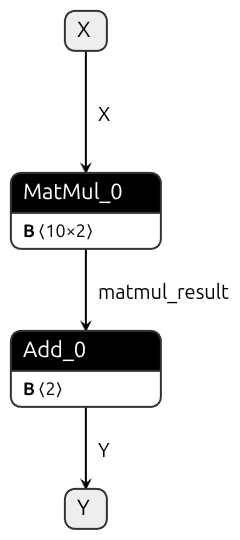
\includegraphics[height=5cm]{imgs/simple_net.onnx.png}
    \end{minipage}
    \caption{An example of a \vnnlib{} query over the real numbers, which explicitly gives the solver permission to (unsoundly) interpret the models from the network theory~$\networkTheoryVar$ as functions over \real. In reality, the network may operate over any floating point type.}
    \label{fig:real-simple-query}
\end{figure}

\begin{figure}[t]
\begin{grammar}
<elementType> $_\real$ = \texttt{real}

<tensor> $_\real$ = $(\shapeVar, \real^\shapeVar)$

<model> $_\real$ = <model> $_\networkTheoryVar$
\end{grammar}

\begin{minipage}{0.6\textwidth}
\begin{equation*}
	\inferrule*[Right=(Element$_\real$)]
	{
        r \in \real
	}
	{
        \vdash r : \mathtt{real}
    }
    \hspace{8em}
    \inferrule*[Right=(Tensor$_\real$)]
    {
    }
    {
        \vdash (\shapeVar, \tensorVar) : (\elementTypeVar, \shapeVar)
    }
\end{equation*}
\begin{equation*}
	\inferrule*[Right=(Model$_\real$)]
	{
        \vdash_\networkTheoryVar \modelVar : \modelTypeVar' \\
        \text{shapesIn}(\modelTypeVar) = \text{shapesIn}(\modelTypeVar)
    }
    {
        \vdash \modelVar : \modelTypeVar 
    }
\end{equation*}
\end{minipage}

\begin{minipage}{0.5\textwidth}
\begin{equation*}
\begin{array}{ll}
\semElementType_\real(\mathtt{real})
&= \real
\\
\semTensor_\real (\mathtt{real}, s)
&= \real^s
\\
\semModel_\real (\networkImplementations)
&= \sem{\mathtt{realModel}}_\networkTheoryVar (\networkImplementations)
\end{array}
\end{equation*}
\end{minipage}

\caption{Construction of a $\networkTheoryVar_\real$ from an abstract network theory $\networkTheoryVar$ and an additional function $\sem{\mathtt{realModel}}_\networkTheoryVar$ that returns the semantics of a network model as a function over real numbers.}
\label{fig:real-network-theory}
\end{figure}

The issue is how to define the syntax and semantics of a real-valued query.
Luckily, the notion of a network theory gives us a modular way to do so. In particular, given a network theory $\networkTheoryVar$ and a function $\sem{\mathtt{realModel}}_\networkTheoryVar$ that interprets models in $\networkTheoryVar$ as real-valued functions, we can define a new network theory $\networkTheoryVar_\real$ as shown in \autoref{fig:real-network-theory}. In particular:
\begin{itemize}
\item \textbf{Element types} in $\networkTheoryVar_\real$, consist of a single type, namely \texttt{real}, that has the expected typing rules and is interpreted in the semantics as $\real$.
\item \textbf{Tensors} in $\networkTheoryVar_\real$ are syntactically just mathematical tensors, again with the expected typing rules and semantics.
\item \textbf{Models} - models in $\networkTheoryVar_\real$ are models from the original theory $\networkTheoryVar$. They are well-typed as long as all the input and output tensors are of the same shape, i.e. the actual original element types provided by $\networkTheoryVar$ are irrelevant. The semantics of the model is provided by the function $\sem{\mathtt{realModel}}_\networkTheoryVar$ that we assume we have access to.
\end{itemize}
We can then use this new theory $\networkTheoryVar_\real$, to obtain both the syntax and semantics for queries over $\real$ simply by reparametrising the exsting syntax and semantics defined in the previous sections. \autoref{fig:real-simple-query} shows an example query over $\networkTheoryVar_\real$.

\section{Mechanisation}

A fully formal version of the contents of this chapter, including the syntax, typing rules and semantics has been mechanised in the Agda interactive theorem prover.
This is available via the official Agda-VNNLIB repository~\cite{}. 